\documentclass[10pt]{report}

\usepackage[utf8]{inputenc}
\usepackage[french]{babel}
\usepackage{cancel}
\usepackage{amsmath}
\usepackage{amsfonts}
\usepackage{amssymb}
\usepackage{graphicx}

\begin{document}

\title{Rapport - Devoir 1}
\date{Octobre 2010}
\author{Vincent Foley-Bourgon (FOLV08078309) \and
  Eric Thivierge (THIE09016601)}

\maketitle

\section{Fonctionnement général du programme}

Le programme effectue, dans l'ordre, les opérations suivantes:

\begin{enumerate}
  \item Lecture d'une chaîne.
  \item Détection des erreurs de syntaxe.
  \item Construction d'un arbre syntaxique abstrait.
  \item Évaluation du résultat.
  \item Détection des erreurs de sémantique.
  \item Affichage.
  \item Retour à l'étape 1.
\end{enumerate}


\subsection{Lecture d'une chaîne}

La lecture de la chaîne entrée par l'utilisateur se fait caractère par
caractère.  Cette lecture est entre-mêlée avec la détection d'erreurs
de syntaxe et la construction de l'ASA (décrits ci-dessous).

\subsection{Détection des erreurs de syntaxe}

Aussitôt qu'une erreur de syntaxe est détectée, la fonction qui génère
l'ASA va vider le tampon d'entrée, libérer les structures de données
temporaires et retourner un code d'erreur.

\subsection{Construction d'un arbre syntaxique abstrait}

Lorsqu'un nombre est lu entièrement, il est ajouté à une pile
d'expressions (une structure qui sera définie plus tard).  Lorsqu'un
opérateur est lu, on combine l'opérateur avec les deux dernières
expressions sur la pile, et on ajoute cette nouvelle expression sur la
pile.

\subsection{Évaluation du résultat}

Lorsqu'un ASA est complet, il est parcouru récursivement à partir de
la racine et à chaque noeud, on applique l'opérateur à ses opérandes.

\subsection{Détection des erreurs de sémantque}

Si durant l'évaluation du résultat une division par zéro est détectée,
un code d'erreur est activé.

\subsection{Affichage}

Si l'expression était valide syntaxiquement et sémentiquement, on
affiche sa représentation dans les syntaxes Scheme, C et Postscript
ainsi que le résultat.  Autrement, un message d'erreur indique la
nature du problème de l'expression.


\section{Représentation des ASAs}

Les arbres de syntaxe abstraite sont des arbres binaires où les noeuds
internes sont des opérateurs et les feuilles sont des nombres.

\[
\text{Expression} =
\left\{
\begin{tabular}{l}
  \text{Nombre} \\
  \text{(Opérateur, Expression, Expression)}
\end{tabular}
\right.
\]

Dans l'implémentation en C, cette structure est représenté par le type
suivant:

\begin{verbatim}
struct Expr {
    enum { operand, expr } type;
    union {
        Number number;
        struct BinaryOperator {
            enum Operator operator;
            struct Expr *left;
            struct Expr *right;
        } expression;
    } _;
};
\end{verbatim}

L'union stockera soit un nombre ou une expression binaire comportant
un opérateur et deux sous-expressions.  Le champ \emph{type} indique
quel champ de l'union est présentement stocké en mémoire.


\newpage

\section{Analyse syntaxique}

Les tâches de lecture des caractères, de création de l'ASA et de
détection des erreurs sont entre-mêlées dans la fonction
\emph{GenerateAST}.

\textbf{Tous les états:} un caractère est lu.  S'il s'agit de EOF, on
retourne le code \emph{ec\_eof}.  Si le caractère est invalide, on
vide le tampon d'entrée et on retourne le code
\emph{ec\_invalid\_symbol}.

\textbf{st\_normal:} si le caractère lu est un chiffre, on met sa
valeur numérique dans la variable \emph{number} et on passe à l'état
\emph{st\_number} pour lire un nombre.  Si le caractère est un
opérateur, on tente de dépiler deux expressions de la pile et de les
combiner avec l'opérateur en une nouvelle expression et l'état passe à
\emph{st\_operator}.  S'il n'y a pas suffisament d'expressions sur la
pile, on vide le tampon d'entrée, on libère -- s'il y a lieu -- les
expressions temporairement allouées et on retourne le code
\emph{ec\_invalid\_syntax}.

\textbf{st\_number:} si le caractère lu est un nombre, on met à jour
la variable \emph{number} en multipliant sa valeur par 10 et en ajout
la valeur numérique du caractère lu.  Si le caractère lu est un
opérateur, c'est une erreur de syntaxe; le tampon d'entrée est vidé et
le code \emph{ec\_invalid\_syntax} est retourné.  Si le caractère est
un espace, on construit une nouvelle expression à partir de
\emph{number} et on ajoute cette expression à la pile.

\textbf{st\_operator:} lorsqu'on est dans l'état \emph{st\_operator},
c'est que le caractère précédent était un opérateur.  Si on lit un
chiffre ou un autre opérateur, la syntaxe de l'expression est
invalide.  Le tampon d'entrée est vidé et le code
\emph{ec\_invalid\_syntax} est retourné.  Si le caractère lu est un
espace, on revient dans l'état \emph{st\_normal}.

\textbf{Après la boucle:} s'il reste un seul élément sur la pile, on
le met dans le paramètre \emph{out} et on retourne \emph{ec\_ok},
sinon on retourne \emph{ec\_invalid\_syntax}.  S'il n'y avait pas
d'élément sur la pile, on retourne \emph{ec\_empty\_expression}.

La figure suivante résume le fonctionnement de la fonction \emph{GenerateAST}:

\begin{center}
  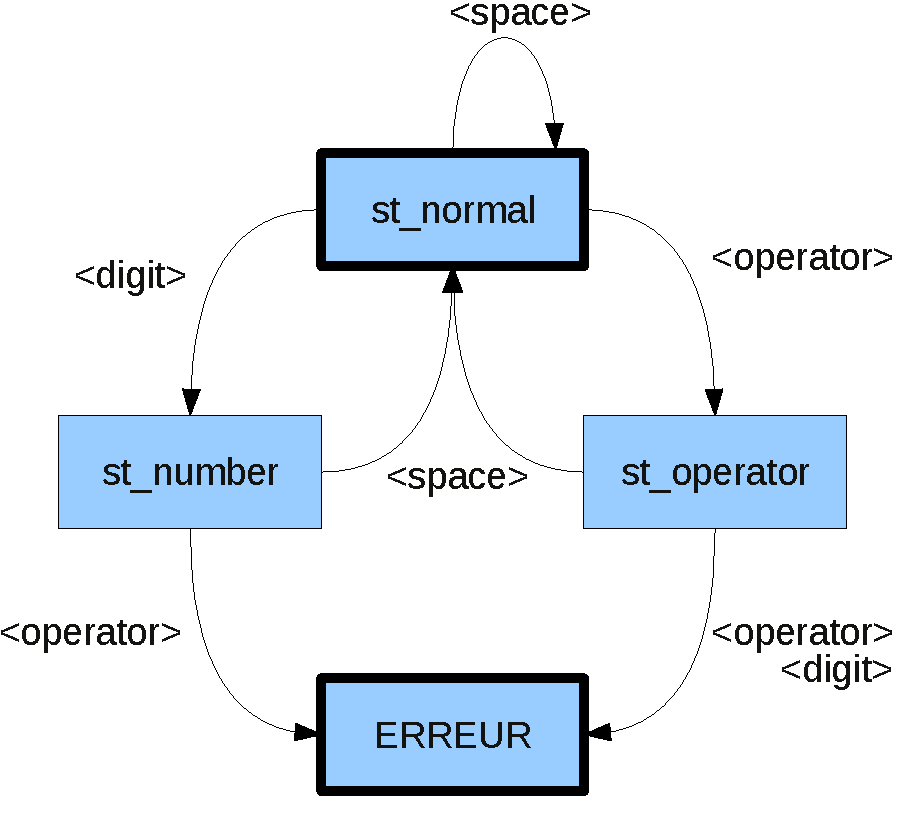
\includegraphics[scale=0.33]{statemachine}
\end{center}



\newpage

\section{Récupération de la mémoire}

La récupération de la mémoire est faite par des fonctions
``destructeurs'' qui vont faire la récupération de leurs éléments
internes.

\textbf{StackFree:} cette fonction parcourt tous les noeuds d'une pile
et appelle \emph{NodeFree} sur ces noeuds.  Lorsque tous les noeuds
ont été récupéré, \emph{StackFree} appelle \emph{free} sur le pointeur
de la pile qui lui a été passé.

\textbf{NodeFree:} cette fonction appelle \emph{ExprFree} sur sa
valeur et appelle ensuite \emph{free} sur le pointeur du noeud qui lui
a été passé.

\textbf{ExprFree:} cette fonction appelle (récursivement)
\emph{ExprFree} sur ses membres de gauche et de droite et appelle
ensuite \emph{free} sur le pointeur de l'expression qui lui a été
passé.

\textbf{StackPop:} dans la fonction \emph{StackPop}, le destructeur
\emph{NodeFree} n'est pas appelé, car il détruirait également
l'expression qu'on veut retourner.  C'est pourquoi il y a un appel
manuel à la fonction \emph{free}.  C'est le seul endroit dans le
programme où une donnée n'est pas détruite par un destructeur.


\end{document}
